\section{Injection models and experiment sets}
\label{sec:injection_models}

\subsection{Overview of simulation and control sets}
\label{sec:simulation_inventory}

We use \emph{deflector} for the foreground lens galaxy in an observed strong
lens and \emph{injection target} for a catalogue galaxy into whose observed
DR10 cutout a simulated lensed source is inserted.
The source family, injection-target population, parameter distribution, noise
treatment, detector, and operating threshold are distinct design axes that can
differ between experiments.
Table~\ref{tab:simulation_sets} summarizes each experiment's question,
population, image construction, and analysis role. Source, target, noise, and
detector settings are specified separately for each experiment. Below,
signal-to-noise ratio is abbreviated as S/N and false-positive rate as FPR. We write
\(p=\operatorname{sigmoid}(\ell)\) for display of a detector's single output
logit \(\ell\); \(p\) is not assumed to be a calibrated probability.

\begin{table*}
\caption{Simulation and control sets used in the study. The visibility
column states the admission policy; absence of an independent visibility cut
retains low-signal configurations. Derived and paired samples reuse the
targets, sources, and scene components indicated in the table.}
\label{tab:simulation_sets}
\centering
{\small
\setlength{\tabcolsep}{2.5pt}
\begin{tabular}{L{0.10\textwidth}L{0.18\textwidth}L{0.20\textwidth}L{0.14\textwidth}L{0.16\textwidth}L{0.15\textwidth}}
\toprule
ID & Question & Source and injection targets & Size & Visibility policy & Analysis role \\
\midrule
$G_{\rm rec}$ &
How often does the primary detector respond over the fixed radius and
observing-condition grid? &
Single S\'{e}rsic sources in catalogue-negative injection targets; source and
lens nuisance draws are shared over radius &
49\,500 injections; 4\,500 distinct targets; nine cells &
No independent S/N or visibility cut &
Fixed-detector recovery and radius curve \\

$G_{\rm domain}$ &
Can the selected observed and injection populations be separated in a fixed
representation? &
Massive-early-type subset of \(G_{\rm rec}\), compared with the 43
selected confirmed systems &
6\,336 injections in 576 targets plus 43 observed systems &
Inherited from \(G_{\rm rec}\) &
Dependency-grouped finite-cohort separation \\

$G_{\rm match}$ &
How does a fixed injection move a matched target along an observed--bare
feature axis? &
Each of the same 43 observed systems and one score-blind matched
\(G_{\rm rec}\) target, using its bare cutout and corresponding
\(\theta_{\rm E}=1.5\)-arcsec injected image &
43 triplets (129 rows) in 43 dependency components &
No post-render selection or target-flux floor &
Cross-fitted representation-axis movement \\

$P_{\rm noise}$ &
How does modelled source-photon sampling change primary-detector response? &
Each \(G_{\rm rec}\) source expectation and eight
\(g=150\ {\rm e^{-}\,nmgy^{-1}}\) Poisson realizations on the same target &
49\,500 deterministic expectation scenes and 396\,000 photon-draw
realizations &
Inherited from \(G_{\rm rec}\); no independent S/N cut &
Photon-minus-expectation paired risk difference \\

$P_{\rm src}$ &
How does the declared structured source construction compare with its
single-S\'{e}rsic twin? &
Restricted high-S/N COSMOS F814W constructions and deterministic catalogue
S\'{e}rsic twins paired on the same \(G_{\rm rec}\) target, with a distinct
target for each pair &
1\,584 pairs; eight draws per pair; 12\,672 paired draw comparisons
(25\,344 arm rows) &
Source-quality restrictions only; no post-render S/N or score cut &
Photon-averaged paired risk difference \\

$C_{\rm bright}$ &
How does response vary with source brightness and photon realization? &
The 43 \(G_{\rm match}\) targets with their stored 1.5-arcsec isolated source
expectations, rescaled to eight magnitudes &
3\,096 derived images and training-preprocessing scores &
No visibility cut; fixed target and geometry &
Fixed-target brightness and source-photon response \\
\bottomrule
\end{tabular}
}
\end{table*}

The recovery set \(G_{\rm rec}\) spans 11 Einstein radii from 0.5 to
3.0~arcsec in 0.25-arcsec steps. Its nine retained \(r\)-band PSF--depth
cells each contain 500 distinct targets, and every target is rendered at all
11 radii. Source, lens-nuisance, colour, and normalized source-offset draws
are shared across radii; only \(\theta_{\rm E}\) and the corresponding
physical source offset vary. The PSF and depth values define descriptive
strata, not interventions.

The experiment retains configurations across the full grid without a
signal-to-noise or visibility threshold, allowing both recovery and failure
to contribute to the conditional response. Population weighting would require
an external distribution over the retained cells.

\(G_{\rm domain}\) reuses a \(G_{\rm rec}\) subset, while \(G_{\rm match}\)
reuses one target's bare and 1.5-arcsec injected pixels per reference. The
primary detector endpoints and \(G_{\rm rec}\), \(P_{\rm noise}\),
\(P_{\rm src}\), and \(C_{\rm bright}\) use the common primary threshold.
The domain and matched analyses instead use continuous cross-fitted readouts
in the four feature protocols.

For \(C_{\rm bright}\), the retained 1.5-arcsec payload for target \(j\) is
decomposed exactly in float32 into bare pixels \(B_j\) and non-negative
source expectation \(S_j\). If its original intrinsic magnitude is \(m_j\),
then at \(m\in\{18.5,19.5,\ldots,25.5\}\)
\begin{equation}
\begin{aligned}
S_{jm}&=10^{-0.4(m-m_j)}S_j,\\
X^{\rm E}_{jm}&=B_j+S_{jm},\\
X^{\rm M}_{jmd}&=B_j+
 \frac{\operatorname{Poisson}(150S_{jm})}{150}.
\end{aligned}
\label{eq:brightness_control}
\end{equation}
There is one expectation and eight keyed photon realizations per
target--magnitude cell. The 3,096 realized images are scored with the
detector's training-consistent 20--32-pixel annulus and clip 10. This scales
an existing lensed source image and does not repeat lens ray-tracing.

\subsection{Injection targets and lens-mass model}
\label{sec:deflector_mass_model}

Injection targets are catalogue-negative objects from the final negative pool
(Section~\ref{sec:sample_provenance}) with valid \(101\times101\)
three-band cutouts and finite cell-assignment quantities. Selection is
score-blind and applies the identity, pixel, within-population spatial-group,
and physical-group role exclusions in Section~\ref{sec:data_partitions}.
Distinct observed references and targets can retain cross-population
geographic links; these remain in the same probe fold
(Section~\ref{sec:linear_probe_methods}). Cells use local Tractor
\texttt{psfsize\_r} and \texttt{psfdepth\_r}, with the latter converted from
inverse-square nanomaggy units to \(5\sigma\) depth. Targets are distinct, but
spatial groups can contain multiple targets across cells; the resampling in
Section~\ref{sec:performance_estimators} preserves these links.

The target roster is selected deterministically without outcomes. Within each
retained PSF--depth cell and spatial group, targets are ordered by a
namespaced SHA-256 hash of cell and galaxy identifier and assigned a
within-group rank. Ranks five and above are removed. The remaining candidates
are ordered first by within-group rank and then by hash, and the first 500
form the cell. A cell is retained only when the candidate roster contains at
least 500 targets and 100 spatial groups and the five-per-group capped
capacity is at least 500.

Within these targets, the operational ``massive early-type'' catalogue
stratum eligible for \(G_{\rm domain}\) requires observed \(z\)-band magnitude
no fainter than 19.5, S\'{e}rsic index at least 4, and catalogue axis ratio at
least 0.6. These cuts select 576 targets and their 6,336 injected scenes.

For \(G_{\rm match}\), each of the 43 selected confirmed systems is assigned
one unique \(G_{\rm rec}\) target by the score-blind matching procedure in
Section~\ref{sec:decomposition_methods}. In contrast, \(P_{\rm src}\) uses
the balanced fixed-scene design in Section~\ref{sec:paired_source_construction},
without matching its targets to observed systems.

Every retained rendering uses a singular isothermal ellipsoid (SIE)
\citep{Kormann1994} with external shear \citep{Keeton2001}. The SIE axis ratio
is drawn from $\mathcal{U}(0.5,1.0)$, its position angle from
$\mathcal{U}(0,\pi)$, the two shear components independently from
$\mathcal{N}(0,0.05^2)$, and the two offsets of the mass centre from
$\mathcal{N}(0,(0.05\;\mathrm{arcsec})^2)$. Numerical treatment near the
circular SIE limit and its validated support are described in
Section~\ref{sec:renderer_validation}.
Einstein radius is the controlled grid axis in \(G_{\rm rec}\),
\(P_{\rm noise}\), and \(P_{\rm src}\). It is fixed at 1.5~arcsec in
\(G_{\rm match}\).

The SIE parameters are assigned independently of an injection target's light,
redshift, velocity dispersion, stellar mass, and environment; axis ratio and
orientation are likewise independent of the observed galaxy shape.
Table~\ref{tab:prematch_coverage} reports actual catalogue
coverage before any matching. The selected systems are substantially brighter
and larger in the central Tractor fit than the \(G_{\rm rec}\) targets. Only
4/4\,500 targets (0.09 per cent) lie jointly within the selected-system
interquartile ranges of \(z\)-band magnitude, half-light radius, and
S\'{e}rsic index. These central-object measurements can include lensed-source
light in the selected systems and therefore describe the measured central
objects rather than deblended deflectors.

\begin{table*}
\caption{Pre-match catalogue coverage of the final \(G_{\rm rec}\) injection
targets and the 43 selected confirmed systems. Numerical rows give the median
[interquartile range] over finite values. The listed quantities are complete
for all 4,500 injection targets. Tractor type counts are SER/DEV/REX/other;
the one selected-system ``other'' object is EXP. These are central-object
catalogue measurements and can include lensed-source light.}
\label{tab:prematch_coverage}
\centering
\begin{tabular}{lrr}
\toprule
Catalogue quantity & \(G_{\rm rec}\) targets (\(N=4\,500\)) &
Selected confirmed systems (\(N=43\)) \\
\midrule
Tractor type counts & 2\,853/1\,213/434/0 & 33/9/0/1 \\
\(r\) magnitude & 20.17 [19.44, 20.84] & 18.16 [17.49, 19.79] \\
\(z\) magnitude & 19.40 [18.71, 19.77] & 17.11 [16.59, 18.32] \\
Half-light radius (arcsec) & 1.05 [0.73, 1.45] & 5.48 [3.63, 7.37] \\
S\'{e}rsic index & 2.60 [1.00, 4.00] & 4.34 [3.68, 5.68] \\
Axis ratio & 0.61 [0.43, 0.78] & 0.70 [0.62, 0.80] \\
\bottomrule
\end{tabular}
\end{table*}

Redshifts are too sparse to inform mass assignment, so the experiment
represents a specified image-generation distribution rather than a calibrated
deflector population. Complex mass structure, line-of-sight perturbers, and
multiple deflectors are not varied as separate factors. Matching uses the five
recorded central-object and observing quantities specified in
Section~\ref{sec:decomposition_methods}.

\subsection{Source models}
\label{sec:source_models}

The parametric source in $G_{\rm rec}$ is a single elliptical S\'{e}rsic
profile \citep{Sersic1968}, with the approximation of
\citet{CiottiBertin1999}, \(b_n=2n-1/3\), used for the S\'{e}rsic constant.
Its unlensed
$r$-band magnitude is drawn uniformly from 23 to 26~mag, S\'{e}rsic index
from $\mathcal{U}(0.5,2.0)$, effective radius from
$\mathcal{U}(0.15,0.50)$~arcsec, axis ratio from
$\mathcal{U}(0.3,1.0)$, and position angle from
$\mathcal{U}(0,2\pi)$. The source offset is expressed as
$\beta_{\rm frac}=\beta/\theta_{\rm E}$ and drawn uniformly in source-plane
area,
\begin{equation}
U_\beta\sim\mathcal{U}(\beta_{\rm lo}^{2},\beta_{\rm hi}^{2}),
\qquad
\beta_{\rm frac}=\sqrt{U_\beta},
\end{equation}
with \((\beta_{\rm lo},\beta_{\rm hi})=(0.10,0.40)\). The same underlying
source and lens draw is inherited without alteration by \(G_{\rm match}\) and
\(P_{\rm noise}\).
\(P_{\rm src}\) inherits the target, lens mapping, source position, and
intrinsic per-band flux but replaces these parametric source-shape
parameters with its paired source constructions.
Independently of the profile's position angle, the polar angle of the
source-centre offset is drawn uniformly from
$\mathcal{U}(0,2\pi)$.
The offset is scaled by the nominal \(\theta_{\rm E}\), not by the realised
caustic of the SIE-plus-shear mapping. Together, these source-position and
lens-model priors determine whether a scene forms a double, quad, or ring.

The parametric colours follow
\(g-r\sim\mathcal{N}(1.15,0.30^2)\) and
\(r-z\sim\mathcal{N}(0.85,0.20^2)\). These values were chosen using
observer-frame annular photometry from 388 of the 389 literature-reviewed
catalogue records. The measured annular means and standard deviations
were $1.23$ and $0.39$ in $g-r$, and $0.95$ and $0.27$ in $r-z$;
the adopted values are design priors rather than direct population estimates.
The catalogue is heterogeneous and the annuli can contain deflector light.

For \(P_{\rm src}\), the structured source-plane construction is drawn from
the GalSim COSMOS 25.2 F814W real-galaxy sample
\citep{Scoville2007,Koekemoer2007,Mandelbaum2012,Rowe2015}.\footnote{The
archived dataset is \citet{Mandelbaum2012},
\url{https://doi.org/10.5281/zenodo.3242143}.} Eligibility requires
elliptical-Gaussian catalogue S/N of at least 100, mask distance of at least
15 native pixels, \(17.0\leq{\tt MAG\_AUTO}\leq24.5\), circularised
half-light radius 0.12--0.60~arcsec, S\'{e}rsic index 0.5--2.0, axis ratio
0.2--1.0, a viable finite single-S\'{e}rsic fit, and measured native inscribed
support of at least six circularised half-light radii. For the COSMOS 25.2
fit catalogue, the single-S\'{e}rsic status is the fifth component
(zero-based index 4) of \texttt{FIT\_STATUS}; codes 0 and 5 are excluded.
No detector output enters eligibility or selection.

The structured profile uses the GalSim \texttt{RealGalaxy} deconvolution of
the observed F814W stamp, with no noise padding, followed by reconvolution to
a common circular Gaussian of 0.15-arcsec FWHM. This scale is broader than
the original F814W PSF for every eligible source. The deterministic twin uses
the same object's catalogue S\'{e}rsic index, circularised half-light radius,
axis ratio, and position angle and is convolved to the same 0.15-arcsec
resolution. Both receive the same source-specific random rotation. They are
drawn on a \(161\times161\) grid with 0.03-arcsec pixels.

After the common low-pass operation, both maps are clipped to non-negative
surface brightness, shifted to the geometric grid centre with a
\(3\times10^{-4}\)-arcsec tolerance, and zeroed outside the same circular
support. That support is 95 per cent of the measured native inscribed radius,
capped at 2.35~arcsec. Each arm must retain at least 90 per cent of its
pre-projection positive flux; the allowed pre-projection
negative-to-positive flux ratios are 0.20 for the structured map and 0.001
for the S\'{e}rsic map. Each projected map is separately normalised to unit
discrete source-plane integral.

The 770 eligible sources are stratified by a \(4\times4\) crossing of
circularised half-light-radius and single-S\'{e}rsic-fit-residual quantiles.
The residual variable is the catalogue-provided \texttt{FIT\_MAD\_S}
statistic for the single-S\'{e}rsic fit.
Within each stratum, a namespaced SHA-256 ordering is computed from the COSMOS
identifier. Ranks 0--8 form the 144-source experiment set and ranks 9--17 form
the disjoint 144-source design set. One F814W spatial map is
constructed for each arm and scaled by the inherited intrinsic flux
in each of \(g,r,z\). Thus each arm reuses its own spatial map across the
three bands. The construction is therefore achromatic, and the structured
arm retains the F814W measurement uncertainty propagated through its
preparation.

\subsection{Ray tracing, flux, PSF, and image construction}
\label{sec:image_construction}

For each injection, we evaluate
\begin{equation}
\boldsymbol{\beta}
=
\boldsymbol{\theta}
-\boldsymbol{\alpha}_{\rm SIE}(\boldsymbol{\theta})
-\boldsymbol{\alpha}_{\rm shear}(\boldsymbol{\theta})
\label{eq:lens_equation}
\end{equation}
where the SIE deflection includes the stated mass-centre offset and the shear
deflection uses the two sampled shear components. Gravitational lensing
conserves surface brightness, not total flux
\citep{NarayanBartelmann1996}. The source model is normalised to its specified
unlensed flux, its surface brightness is evaluated at the ray-traced
source-plane positions, and the image-plane flux is allowed to change under
the resulting magnification; the lensed image is never renormalised.

For \(G_{\rm rec}\), tensor Gauss--Legendre quadrature integrates the
analytic S\'{e}rsic surface brightness over each native
0.262-arcsec pixel. The analytic elliptical-S\'{e}rsic integral sets the
unlensed per-band flux. Orders 24 and 32 provide the registered per-scene
comparison: the unlensed-flux relative error must be at most 0.01, the
successive lensed-image relative \(L_1\) difference at most 0.005, and the
relative peak difference at most 0.02. One retained scene required the
score-blind order-48 extension.

We approximate the local PSF in each band by a circular Gaussian. Its
\(r\)-band FWHM is
taken from the injection target's Tractor \texttt{psfsize\_r} value; the
\(g\)- and \(z\)-band FWHM values are set to 1.05 and 0.94 times the \(r\)-band
value, respectively. These fixed ratios are renderer approximations rather
than per-target measurements of the $g$- and $z$-band PSFs. The rendered
lensed source is converted to nanomaggies per native pixel and convolved
after pixel integration on the native grid. The Gaussian kernel is truncated
at \(8\sigma\), and explicit zero padding prevents periodic wrap-around.
The renderer therefore uses a circular effective post-pixel coadd PSF;
exposure-level optical structure and PSF anisotropy are outside this model.
The result is added to the observed
injection-target cutout before the preprocessing in
Section~\ref{sec:preprocessing}. The target cutout therefore remains the
same within a controlled pair.

The \(G_{\rm match}\) injected member is the exact stored
\(\theta_{\rm E}=1.5\)-arcsec \(G_{\rm rec}\) deterministic expectation array, and its bare
member is the exact stored target cutout; neither arm is rerendered or
flux-rescaled. For \(P_{\rm src}\), each non-parametric source map is
bilinearly interpolated with zero outside its recorded support on a grid
oversampled by a factor of eight in each image dimension. Surface brightness
is block-averaged to native pixels, multiplied by the fixed inherited intrinsic
per-band flux and native-pixel area, and then convolved with the same
zero-padded effective post-pixel Gaussian. The \(4\times\), \(8\times\), and
\(16\times\) renderings of every final pair must have consecutive relative
\(L_1\) differences below 0.01; the maximum in the final bank is 0.0022.
These comparisons assess numerical integration at the fixed DR10 pixel scale
and effective PSF.

\subsection{Noise model}
\label{sec:noise_model}

An observed DR10 injection-target cutout already contains foreground light and
realised sky, detector, coaddition, and survey-processing noise. The stored
\(G_{\rm rec}\) expectation adds rendered source light without an additional
source-photon or sky-noise field. \(P_{\rm noise}\) and \(P_{\rm src}\) add
only the modelled source-photon realization; neither redraws the target's
existing noise.

For non-negative injected-source expectation \(I\) in nanomaggies per native
pixel and a modelled conversion \(g\) in electrons per nanomaggy,
\(P_{\rm noise}\) draws
\begin{equation}
\begin{aligned}
 E&=g\max(I,0),&
 E'&\sim\operatorname{Poisson}(E),\\
 I_{\rm photon}&=\frac{E'}{g}
 =I+\frac{E'-E}{g}.
\end{aligned}
\label{eq:poisson_arc_noise}
\end{equation}
Pixels with zero injected flux therefore receive zero source counts. We use
\(g=150\;\mathrm{e^{-}\,nmgy^{-1}}\) as a modelled conversion, not as a
calibrated gain for every contributing DR10 exposure. One independent
PCG64DXSM stream is derived by SHA-256 from each scene and draw identity.
Every deterministic expectation scene receives eight draws, each added to the
exact stored target bytes.

A separate pilot, conducted without detector scores, was used to choose the
number of photon realizations. Appendix
Table~\ref{tab:pnoise_draw_pilot} reports the pilot sample, the tested draw
counts, and their Monte Carlo standard errors (MCSEs).

The \(P_{\rm src}\) arms use the same modelled \(g=150\) conversion but couple
their Poisson draws. For structured and S\'{e}rsic expected electron
intensities \(\lambda_{\rm str}=gI_{\rm str}\) and
\(\lambda_{\rm ser}=gI_{\rm ser}\), let
\(\lambda_{\rm min}=\min(\lambda_{\rm str},\lambda_{\rm ser})\) pixelwise.
The construction draws
\begin{equation}
\begin{aligned}
 C&\sim{\rm Poisson}(\lambda_{\rm min}),\\
 A&\sim{\rm Poisson}(\lambda_{\rm str}-\lambda_{\rm min}),\qquad
 B\sim{\rm Poisson}(\lambda_{\rm ser}-\lambda_{\rm min}),\\
 I'_{\rm str}&=(C+A)/g,\qquad I'_{\rm ser}=(C+B)/g ,
\end{aligned}
\label{eq:coupled_source_photons}
\end{equation}
using three independent keyed streams. Each arm retains its exact Poisson
marginal; equal expected intensities produce identical counts, while only the
excess intensity is drawn independently.

The F814W measurement uncertainty retained by the structured
\(P_{\rm src}\) map is distinct from the source-photon draw.

Figure~\ref{fig:final_psrc_construction} illustrates both source
constructions at the expectation and photon-realized stages.

\begin{figure*}
\centering
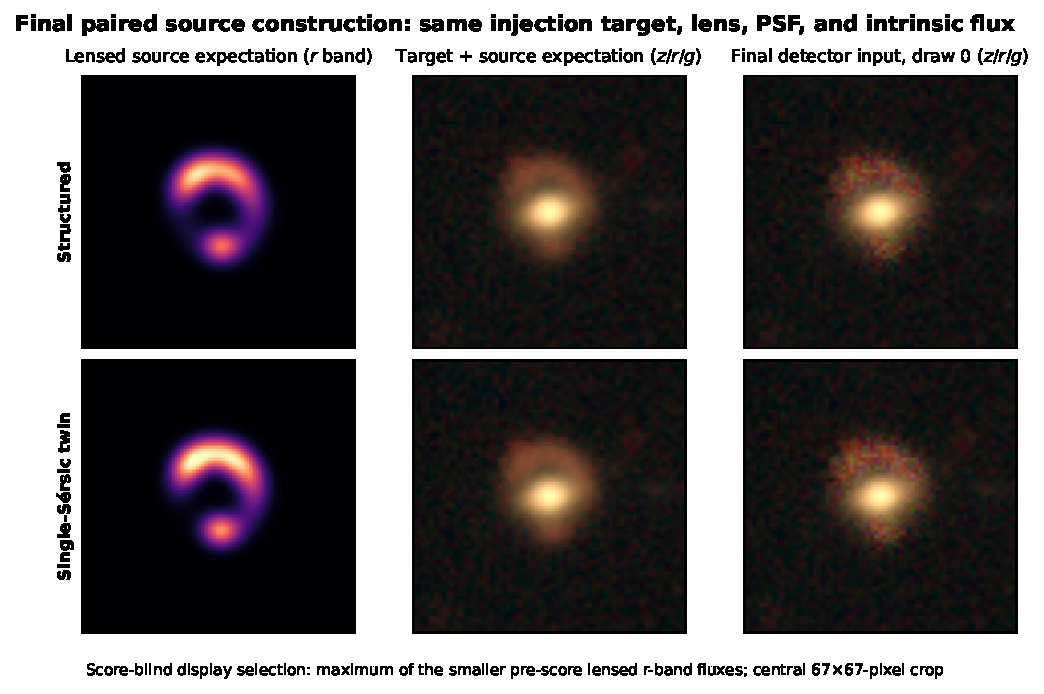
\includegraphics[width=\textwidth]{figures/section3_final_psrc_construction.pdf}
\caption{Illustration from the final \(P_{\rm src}\) bank. The pair is selected
without detector scores by maximizing the smaller of the two pre-score lensed
\(r\)-band fluxes, solely to make the inserted light visible. This display
selection does not alter the analysis population; the pair remains in the
final paired analysis. Rows show the structured
construction and its deterministic single-S\'{e}rsic twin. Columns show the
lensed source expectation in \(r\), the target plus source expectation in
\(z/r/g\) colour, and final photon draw 0 supplied to the detector. The pair
shares the target, source identity, lens mapping, nominal source-plane centre,
effective PSF, intrinsic per-band flux, and photon coupling, but receives no post-lensing
flux rescaling. Panels use the central \(67\times67\)-pixel display crop; the
detector uses all \(101\times101\) pixels.}
\label{fig:final_psrc_construction}
\par\smallskip{\raggedright\noindent\textit{Alt text:} Two rows compare the structured
source and its smooth single-S\'{e}rsic twin. The first column shows similar
but visibly non-identical ring-like \(r\)-band source expectations. The second
shows each expectation added to the same bright central survey galaxy. The
third shows photon draw 0, where coupled source-photon fluctuations are
visible around the shared foreground scene.\par}
\end{figure*}

\subsection{Paired source construction}
\label{sec:paired_source_construction}

The final \(P_{\rm src}\) design has 99 target-cell--radius blocks. Each block
contains 16 distinct targets, with four from each within-cell
intrinsic-\(r\)-magnitude quantile and one assignment from each source
stratum. This gives 1,584 pairs on distinct targets; each of the 144 empirical
sources is used 11 times.

Targets are ordered by a namespaced SHA-256 hash within each cell and
intrinsic-magnitude quantile before four are assigned to each radius. Parent
scenes are then ordered within cell--radius blocks, and the 16 source strata
are cycled deterministically across those blocks using the hash-ordered source
rosters. The assignment uses no detector score, threshold decision, or probe
feature.

Within a pair, the structured and deterministic single-S\'{e}rsic maps share
the exact target, lens and shear parameters, source position,
aligned source-plane centroid, effective per-band PSF, intrinsic \(g/r/z\) fluxes,
renderer, and photon draw indices. The primary design fixes intrinsic flux
before lensing and applies no post-lensing rescaling. Differences in
magnification induced by the two source maps therefore remain part of the
source-construction intervention. The realised flux centroids are not explicitly aligned
after rendering.

A separate design pilot uses disjoint targets and sources under the same
cell, radius, magnitude, and source-stratum structure. Eight is the smallest
tested draw count meeting its paired-risk MCSE criterion; Appendix
Table~\ref{tab:psrc_draw_pilot} gives the candidate panel.

The comparison in Section~\ref{sec:paired_source_estimators} therefore
isolates the two complete source-construction pathways at the same intrinsic
flux and nominal source-plane centre.

\subsection{Renderer validation}
\label{sec:renderer_validation}

A stratified 142-scene audit evaluates quadrature, an independently refined
integration, an effective-PSF reference, and SIE deflections from Lenstronomy
\citep{Birrer2018}. Appendix~\ref{app:renderer_reconciliation} reports its
support and numerical bounds. These tests assess numerical accuracy for the
configurations examined; they do not test whether the adopted source, lens,
PSF, or detector models are astrophysically complete.
